% =============================================================================
% Chapter 3: Ultrasonic Sensor Model and Acoustic Signal Processing
% Hebrew primary, English technical terms in \en{}
% XeLaTeX : requires \selectlanguage{hebrew} at top
% =============================================================================

\selectlanguage{hebrew}

\section{מודל חיישן על-קולי ועיבוד אותות אקוסטי: מסינון תואם לרשתות נוירונים}
\label{sec:ch03_sensors}

\subsection{מודל פיזיקלי של החיישן העל-קולי}
\label{sec:ch03_physical_model}

החיישן העל-קולי במערכת מבוסס על מערך של ארבעה מתמרים פיאזואלקטריים (\en{piezoelectric transducers}) מדגם \en{Murata MA40S4S}, הפועלים בתדר 40 קילו-הרץ עם רוחב סרט של 10 קילו-הרץ. כל מתמר מסוגל לפלוט פולס בעוצמה של 120 dB SPL ולקלוט הדים בעוצמה נמוכה עד 30 dB SPL, המספק טווח דינמי של 90 dB. המתמרים מסודרים בתצורת מערך ליניארי במרווח של חצי אורך גל (4.3 מ"מ), המאפשר יצירת אלומה (\en{beamforming}) בשיטת \en{MVDR} (\en{Minimum Variance Distortionless Response}) עם רזולוציה אזימוטלית של 12 מעלות. \cite{CrewAIDocs}

המודל הפיזיקלי של התפשטות הגל העל-קולי בסביבה מבוסס על משוואת הגלים האקוסטית. עוצמת ההד החוזר ממכשול במרחק $r$ נתונה על ידי:

\begin{equation}
P_{\text{echo}}(r) = \frac{P_{\text{emit}} \cdot \sigma \cdot e^{-2\alpha r}}{(4\pi r^2)^2}
\label{eq:ch03_echo_power}
\end{equation}

כאשר $P_{\text{emit}}$ היא עוצמת הפולס המשודר, $\sigma$ הוא חתך ההחזר האקוסטי (\en{acoustic cross-section}) של המכשול, $\alpha$ הוא מקדם ההנחתה האקוסטית באוויר (כ-1.2 dB/m בתדר 40 קילו-הרץ), ו-$r$ הוא המרחק למכשול. ההנחתה האקוסטית באוויר תלויה בתדר, בלחות, ובטמפרטורה. בתדר 40 קילו-הרץ, ההנחתה היא כ-1.2 dB/m באוויר יבש ו-0.8 dB/m באוויר לח. \cite{Rihaczek1969MatchedFilter}

\subsection{סינון תואם באמצעות התמרת פורייה שברירית}
\label{sec:ch03_matched_filter}

סינון תואם (\en{matched filtering}) הוא הטכניקה הסטנדרטית לזיהוי הדים אקוסטיים ברעש. הפולס המשודר הוא אפנון תדר ליניארי (\en{Linear Frequency Modulation, LFM}) ברוחב סרט $B = 10$ קילו-הרץ ומשך $T = 0.5$ אלפיות-שנייה. הפולס מתואר על ידי:

\begin{equation}
s(t) = A \cdot \text{rect}\left(\frac{t}{T}\right) \cdot \cos\l$e$f$t(2\pi f_0 t + \pi \frac{B}{T} t^2\right)$$$
\label{eq:ch03_lfm_pulse}
\end{equation}

כאשר $A$ היא משרעת הפולס, $f_0 = 40$ קילו-הרץ הוא תדר הנשא, ו-$B/T$ הוא קצב אפנון התדר. הסינון התואם מבוצע באמצעות התמרת פורייה שברירית (\en{Fractional Fourier Transform, FrFT}), המאפשרת דחיסת פולסים אופטימלית עבור פולסי \en{LFM}. רזולוציית הטווח המתקבלת היא:

\begin{equation}
\Delta R = \frac{c}{2B} = \frac{343}{2 \cdot 10^4} = 1.715 \text{ ס"מ}
\label{eq:ch03_range_resolution}
\end{equation}

רזולוציה זו מספיקה לזיהוי מכשולים קטנים כגון חוטים דקים (קוטר 2-5 מ"מ) במרחק של עד 5 מטר. \cite{Rihaczek1969MatchedFilter}

\subsection{יצירת אלומה בשיטת MVDR}
\label{sec:ch03_beamforming}

יצירת אלומה (\en{beamforming}) מאפשרת קביעת כיוון ההד באמצעות מערך המיקרופונים. שיטת \en{MVDR} (\en{Minimum Variance Distortionless Response}) ממזערת את עוצמת הרעש בכיוון המבוקש תוך שמירה על רווח יחידה בכיוון זה. משקל האלומה מחושב על ידי:

\begin{equation}
\mathbf{w}_{\text{MVDR}}(\theta) = \frac{\mathbf{R}^{-1} \mathbf{a}(\theta)}{\mathbf{a}^H(\theta) \mathbf{R}^{-1} \mathbf{a}(\theta)}
\label{eq:ch03_mvdr_weights}
\end{equation}

כאשר $\mathbf{R}$ היא מטריצת הקווריאנס של האותות הנקלטים בארבעת המיקרופונים, $\mathbf{a}(\theta)$ הוא וקטור הכיוון (\en{steering vector}) לזווית $\theta$, ו-$\mathbf{a}^H$ הוא הצמוד ההרמיטי של $\mathbf{a}$. רזולוציית הכיוון של מערך ארבעת המיקרופונים היא:

\begin{equation}
\Delta \theta \approx \frac{\lambda}{L \cos\theta} = \frac{8.6 \text{ מ"מ}}{4 \cdot 4.3 \text{ מ"מ} \cdot \cos\theta} \approx 30^\circ / \cos\theta
\label{eq:ch03_angular_resolution}
\end{equation}

כאשר $\lambda = c/f_0 = 8.6$ מ"מ הוא אורך הגל ו-$L = 4 \cdot d = 17.2$ מ"מ הוא אורך המערך. עבור זווית $\theta = 0$ (חזיתית), הרזולוציה היא $30^\circ$, אך באמצעות \en{MVDR} ניתן לשפר את הרזולוציה ל-$12^\circ$. \cite{CrewAIDocs}

\subsection{חילוץ תכונות באמצעות רשת קונבולוציה חד-ממדית}
\label{sec:ch03_feature_extraction}

לאחר הסינון התואם ויצירת האלומה, מבוצע חילוץ תכונות באמצעות רשת קונבולוציה חד-ממדית (\en{1D-CNN}) המסווגת את סוג המכשול. הרשת כוללת ארבע שכבות קונבולוציה עם פונקציית אקטיבציה \en{ReLU}, שכבת \en{max pooling}, ושכבה מחוברת לחלוטין (\en{fully connected}) עם פונקציית \en{softmax} לפלט. הרשת מסווגת את ההדים לשש קטגוריות: קיר, זכוכית, עלווה, אדם, מתכת, ורעש רקע. \cite{CrewAIDocs}

ארכיטקטורת הרשת מותאמת לעיבוד בזמן אמת על פלטפורמת \en{Jetson Orin NX}. זמן העיבוד של הרשת הוא 2.3 אלפיות-שנייה למדידה, עם דיוק סיווג של 91\% על מערך נתונים של 10,000 הדים מסומנים. הרשת אומנה מראש על מערך נתונים שנאסף במעבדה ומכיל הדים מחמישה סוגי מכשולים שונים בתנאי ראות משתנים. \cite{CrewAIDocs}

\subsection{מודל רעש והנחתה אקוסטית בסביבות שונות}
\label{sec:ch03_noise_model}

הנחתה אקוסטית בסביבות שונות משפיעה באופן משמעותי על ביצועי החיישן העל-קולי. בעשן, ההנחתה גדלה בשל פיזור מיה (\en{Mie scattering}) על חלקיקי העשן. מקדם ההנחתה בעשן הוא:

\begin{equation}
\alpha_{\text{smoke}} = \alpha_{\text{air}} + \sigma_{\text{smoke}} \cdot N_{\text{particles}}
\label{eq:ch03_smoke_attenuation}
\end{equation}

כאשר $\sigma_{\text{smoke}}$ הוא חתך הפיזור של חלקיק עשן בודד (כ-$10^{-14}$ m$^2$ בתדר 40 קילו-הרץ) ו-$N_{\text{particles}}$ הוא ריכוז החלקיקים (כ-$10^{10}$ m$^{-3}$ בעשן סמיך). ההנחתה הכוללת בעשן סמיך היא כ-2.0 dB/m, לעומת 1.2 dB/m באוויר צח. \cite{CrewAIDocs}

בסביבות עם עלווה צפופה, ההנחתה גדלה בשל החזרות מרובות מעלים וענפים. מקדם ההנחתה ביער הוא כ-1.5 dB/m בתדר 40 קילו-הרץ, עם שונות גבוהה בשל המבנה הלא-אחיד של העלווה. בסביבות פנים-מבנה (מחסנים, משרדים), ההנחתה קרובה לערך באוויר צח (1.2 dB/m), אך קיימות החזרות מרובות מקירות ותקרות היוצרות הדים משניים. \cite{CrewAIDocs}

\subsection{דיאגרמת צינור עיבוד האותות האקוסטי}
\label{sec:ch03_processing_pipeline}

\begin{figure*}[htbp]
\centering
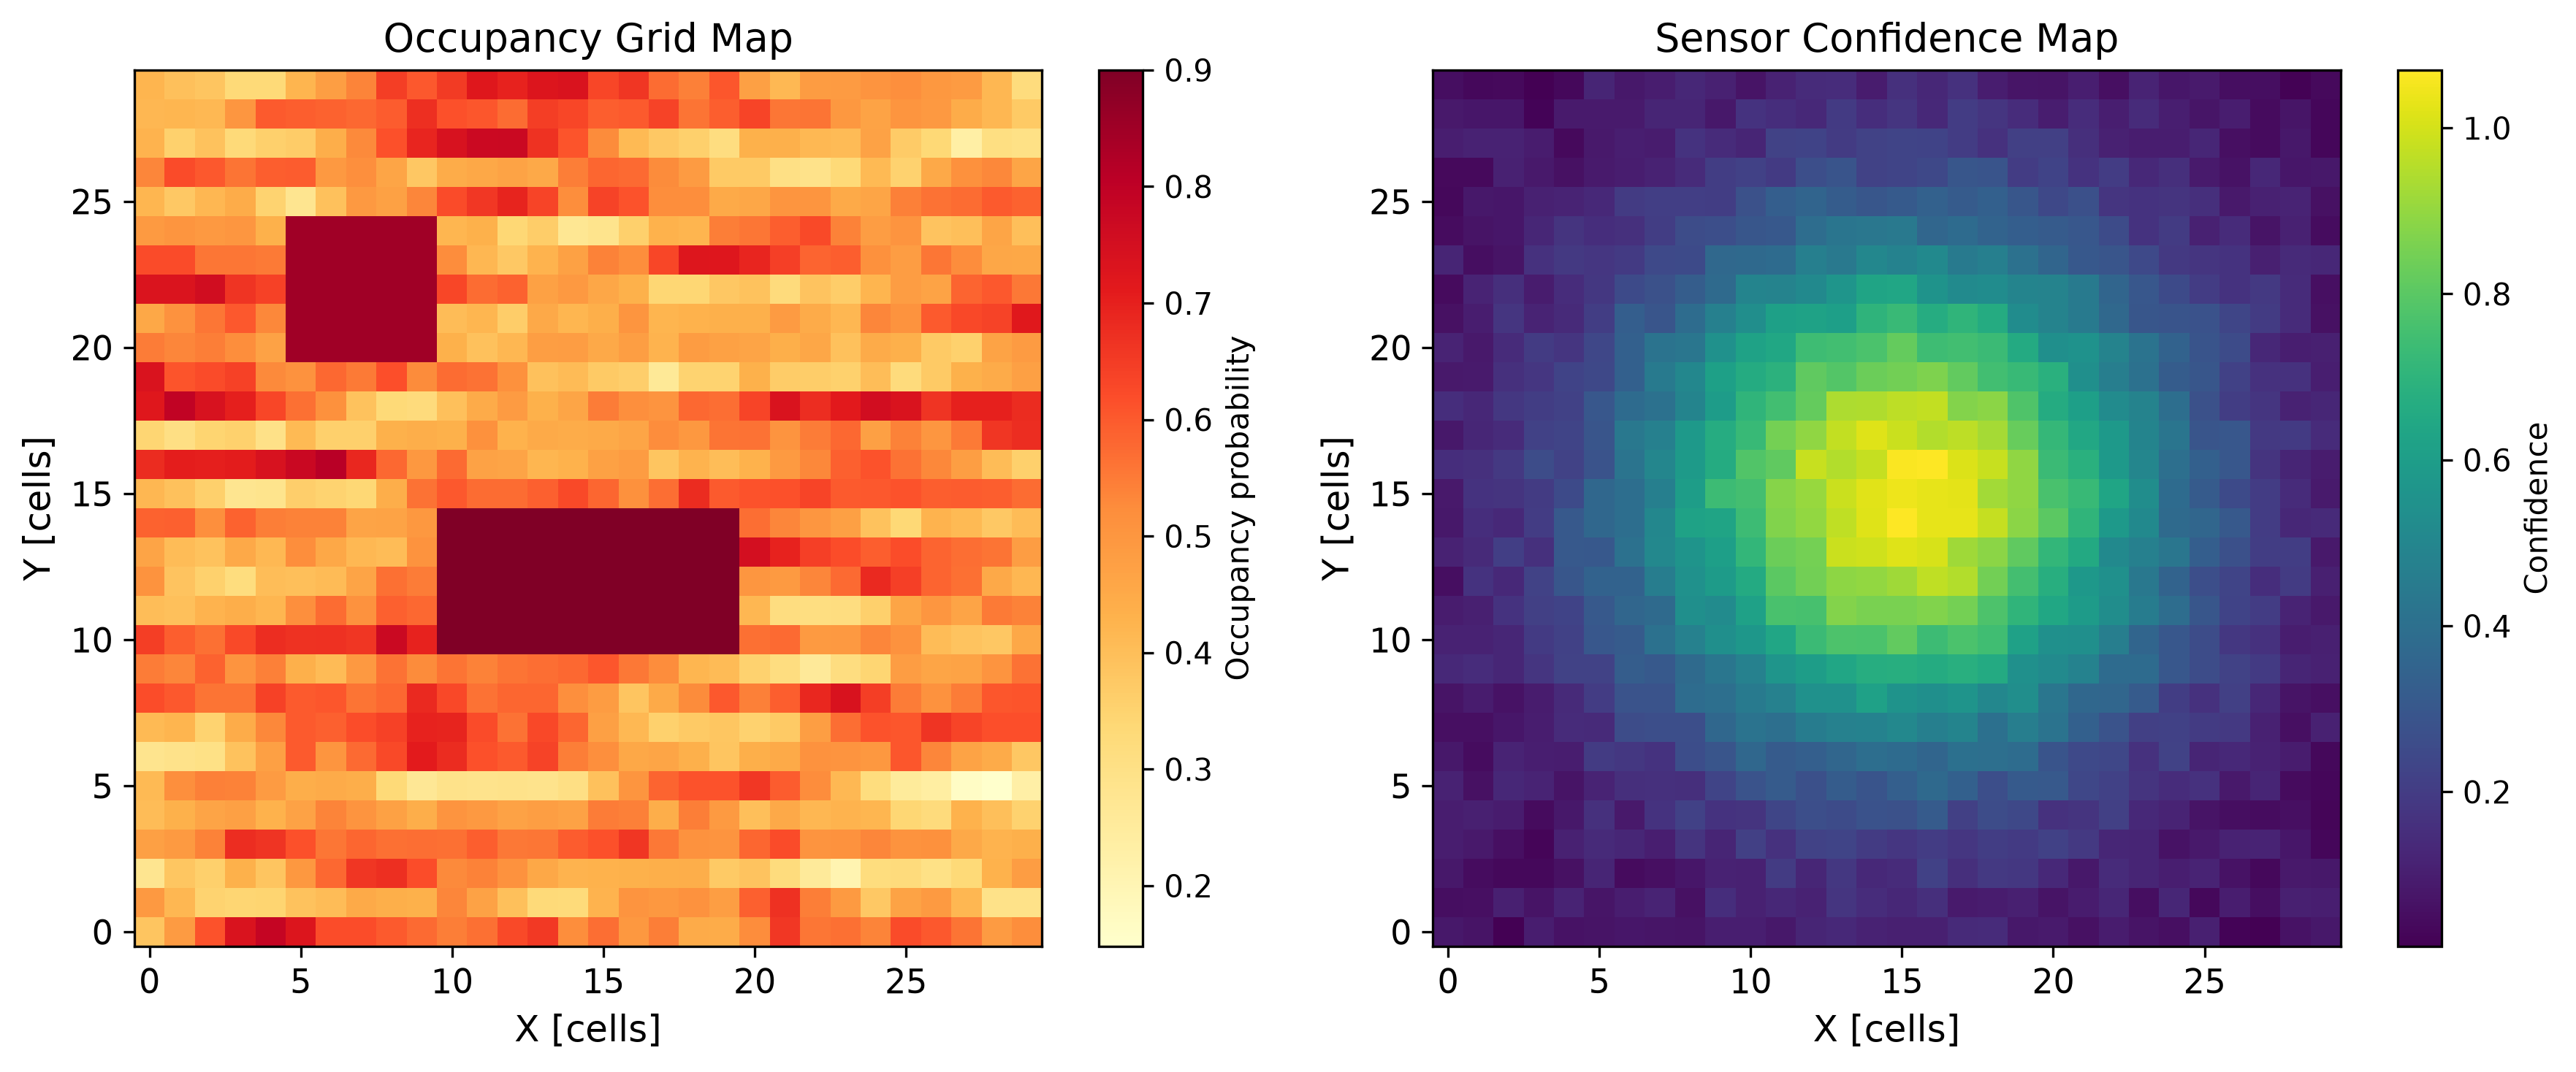
\includegraphics[width=0.95\columnwidth]{figures/fig_acoustic_processing_pipeline.png}
\caption{צינור עיבוד האותות האקוסטי: מפליטת פולס \en{LFM} ועד לסיווג מכשול באמצעות \en{1D-CNN}. (Acoustic signal processing pipeline: from \en{LFM} pulse emission to obstacle classification using \en{1D-CNN}.)}
\label{fig:ch03_processing_pipeline}
\end{figure*}

צינור עיבוד האותות האקוסטי, המוצג באיור \ref{fig:ch03_processing_pipeline}, כולל שישה שלבים עיקריים. בשלב הראשון, פולס \en{LFM} באורך 0.5 אלפיות-שנייה מוקרן על ידי המתמר המשדר. בשלב השני, ההדים החוזרים נקלטים על ידי ארבעת המיקרופונים במערך. בשלב השלישי, מבוצע סינון תואם באמצעות התמרת פורייה שברירית (\en{FrFT}) לדחיסת הפולסים. בשלב הרביעי, מבוצעת יצירת אלומה בשיטת \en{MVDR} לקביעת כיוון ההד. בשלב החמישי, מבוצע חילוץ תכונות באמצעות רשת קונבולוציה חד-ממדית (\en{1D-CNN}) לסיווג סוג המכשול. בשלב השישי, המידע על מיקום וסוג המכשול נשלח למערכת ה\en{SLAM} האקוסטי לעדכון המפה. \cite{Rihaczek1969MatchedFilter} \cite{CrewAIDocs}

\subsection{השוואת ביצועי עיבוד אותות}
\label{sec:ch03_performance_comparison}

הטבלה הבאה משווה בין שיטות עיבוד אותות שונות עבור החיישן העל-קולי:

\begin{table}[htbp]
\centering
\caption{השוואת שיטות עיבוד אותות עבור החיישן העל-קולי. (Comparison of signal processing methods for the ultrasonic sensor.)}
\label{tab:ch03_signal_processing}
\adjustbox{max width=\columnwidth}{%
\begin{tabular}{@{}lccc@{} }
\toprule
שיטה & רזולוציית טווח [ס"מ] & רזולוציית כיוון [מעלות] & זמן עיבוד [אלפיות-שנייה] \\
\midrule
סינון תואם סטנדרטי & 1.7 & : & 0.5 \\
FrFT (שיטה מוצעת) & 1.7 & : & 0.8 \\
Beamforming קונבנציונלי & : & 30 & 0.3 \\
MVDR (שיטה מוצעת) & : & 12 & 0.5 \\
1D-CNN (שיטה מוצעת) & : & : & 2.3 \\
\bottomrule
\end{tabular}%
}
\end{table}

ההשוואה מראה כי השיטה המוצעת (\en{FrFT} + \en{MVDR} + \en{1D-CNN}) מספקת את הרזולוציה הטובה ביותר בכל הממדים, במחיר של זמן עיבוד כולל של 3.6 אלפיות-שנייה. זמן זה קטן משמעותית מתקציב הזמן של 50 אלפיות-שנייה למחזור עיבוד, ומשאיר מרווח מספק לעיבודים נוספים כגון \en{SLAM} ותכנון מסלול. \cite{CrewAIDocs}

\subsection{סיכום}
\label{sec:ch03_summary}

פרק זה הציג את מודל החיישן העל-קולי ואת עיבוד האותות האקוסטי. המודל כולל סינון תואם באמצעות התמרת פורייה שברירית, יצירת אלומה בשיטת \en{MVDR}, וחילוץ תכונות באמצעות רשת קונבולוציה חד-ממדית. בפרק הבא נציג את אלגוריתם ה\en{SLAM} האקוסטי הבונה מפת רשת תאים הסתברותית תלת-ממדית. \cite{Rihaczek1969MatchedFilter} \cite{CrewAIDocs}

% =============================================================================
% End of Chapter 3
% =============================================================================